\documentclass[a4paper,11pt]{article}



\usepackage{cmap}					% поиск в PDF
\usepackage[T2A]{fontenc}			% кодировка
\usepackage[utf8]{inputenc}			% кодировка исходного текста
\usepackage[english,russian]{babel}	% локализация и переносы
\usepackage{geometry}
\usepackage{setspace,amsmath}
\usepackage{verbatim}
\usepackage{graphicx}
\usepackage{hyperref}

\usepackage{cmap}					% поиск в PDF
\usepackage{mathtext} 				% русские буквы в формулах
\usepackage[T2A]{fontenc}			% кодировка
\usepackage[utf8]{inputenc}			% кодировка исходного текста
\usepackage[english,russian]{babel}	% локализация и переносы
\usepackage{indentfirst}            % красная строка в первом абзаце
\frenchspacing                      % равные пробелы между словами и предложениями

%%% Дополнительная работа с математикой
\usepackage{amsmath,amsfonts,amssymb,amsthm,mathtools} % пакеты AMS
\usepackage{icomma}                                    % "Умная" запятая

%%% Свои символы и команды
\usepackage{centernot} % центрированное зачеркивание символа
\usepackage{stmaryrd}  % некоторые спецсимволы
\usepackage{dsfont}
\usepackage{amsthm}

\renewcommand{\epsilon}{\ensuremath{\varepsilon}}
\renewcommand{\phi}{\ensuremath{\varphi}}
\renewcommand{\kappa}{\ensuremath{\varkappa}}
\renewcommand{\le}{\ensuremath{\leqslant}}
\renewcommand{\leq}{\ensuremath{\leqslant}}
\renewcommand{\ge}{\ensuremath{\geqslant}}
\renewcommand{\geq}{\ensuremath{\geqslant}}
\renewcommand{\emptyset}{\ensuremath{\varnothing}}

\DeclareMathOperator*{\Mid}{\scalebox{1.1}{$\mid$}}

\DeclareMathOperator{\sgn}{sgn}
\DeclareMathOperator{\gd}{\text{НОД}}
\DeclareMathOperator{\lf}{\text{НОК}}
\DeclareMathOperator{\rk}{rk}
\DeclareMathOperator{\pr}{pr}
\DeclareMathOperator{\im}{Im}
\DeclareMathOperator{\ke}{Ker}
\DeclareMathOperator{\re}{Re}
\DeclareMathOperator{\cha}{char}
\DeclareMathOperator{\ord}{ord}
\DeclareMathOperator{\tr}{tr}
\DeclareMathOperator{\md}{mod}
\DeclareMathOperator{\Aut}{Aut}
\DeclareMathOperator{\Inn}{Inn}
\DeclareMathOperator{\End}{End}
\DeclareMathOperator{\GL}{GL}
\DeclareMathOperator{\SL}{SL}
\DeclareMathOperator{\diag}{diag}

\newcommand{\divby}{
	\mathrel{\vbox{\baselineskip.65ex\lineskiplimit0pt\hbox{.}\hbox{.}\hbox{.}}}
}
\newcommand{\notdivby}{\centernot\divby}
\newcommand{\N}{\mathbb{N}}
\newcommand{\Z}{\mathbb{Z}}
\newcommand{\Q}{\mathbb{Q}}
\newcommand{\R}{\mathbb{R}}
\newcommand{\Cm}{\mathbb{C}}
\newcommand{\F}{\mathbb{F}}
\newcommand{\id}{\mathrm{id}}
\newcommand{\imp}[2]{(#1\,\,$\ra$\,\,#2)\,\,}
\newcommand{\nset}[1]{\{1, \dotsc, #1\}}
\newcommand{\Chi}{\scalebox{1.1}{\raisebox{\depth}{$\chi$}}}
\newcommand{\FF}{\scalebox{0.95}{$\mathcal F$}}
\newcommand{\FFF}{\scalebox{0.55}{$\mathcal F$}}
\newcommand{\GG}{\scalebox{0.95}{$\mathcal G$}}
\newcommand{\GGG}{\scalebox{0.55}{$\mathcal G$}}

\renewcommand\labelitemi{$\triangleright$}

\let\bs\backslash
\let\vect\overline
\let\normal\trianglelefteqslant
\let\lra\Leftrightarrow
\let\ra\Rightarrow
\let\la\Leftarrow
\let\gl\langle
\let\gr\rangle
\let\sd\leftthreetimes
\let\emb\hookrightarrow
\let\mc\mathcal
\let\mf\mathfrak

%%% Перенос знаков в формулах (по Львовскому)
\newcommand*{\hm}[1]{#1\nobreak\discretionary{}{\hbox{$\mathsurround=0pt #1$}}{}}

%%% Работа с картинками
\usepackage{graphicx}    % Для вставки рисунков
\setlength\fboxsep{3pt}  % Отступ рамки \fbox{} от рисунка
\setlength\fboxrule{1pt} % Толщина линий рамки \fbox{}
\usepackage{wrapfig}     % Обтекание рисунков текстом

%%% Работа с таблицами
\usepackage{array,tabularx,tabulary,booktabs} % Дополнительная работа с таблицами
\usepackage{longtable}                        % Длинные таблицы
\usepackage{multirow}                         % Слияние строк в таблице

%%% Теоремы
\theoremstyle{plain}
\newtheorem{theorem}{Теорема}[section]
\newtheorem{lemma}{Лемма}[section]
\newtheorem{proposition}{Утверждение}[section]
\newtheorem*{exercise}{Упражнение}
\newtheorem*{problem}{Задача}

\theoremstyle{definition}
\newtheorem{definition}{Определение}[section]
\newtheorem*{corollary}{Следствие}
\newtheorem*{note}{Замечание}
\newtheorem*{reminder}{Напоминание}
\newtheorem*{example}{Пример}
\newtheorem*{remarkfrom}{Примечание авторов}
\newtheorem*{agreement}{Соглашение}
\newtheorem*{idea}{Идея доказательства}
\newtheorem*{algorithm}{Алгоритм}

\theoremstyle{remark}
\newtheorem*{solution}{Решение}

\makeatletter
\renewcommand{\@listI}{%
\topsep=0pt }
\makeatother

\makeatletter
\let\old@itemize=\itemize
\def\itemize{\old@itemize
\setlength{\itemsep}{0pt}
\setlength{\parskip}{0pt}
\setlength{\leftskip}{0pt}
}
\makeatother

\makeatletter
\let\old@enumerate=\enumerate
\def\enumerate{\old@enumerate
\setlength{\itemsep}{0pt}
\setlength{\parskip}{0pt}
\setlength{\leftskip}{0pt}
}\makeatother

\geometry{
  top=15mm, 
  right=10mm, 
  bottom=15mm, 
  left=10mm
}

\author{Андрей Рыжов\\МФТИ, 2024}
\title{Остовное дерево минимальной степени}

\begin{document}

\maketitle

\begin{abstract}
В данном отчете рассмотрена задача поиска остовного дерева минимальной степени, то есть остовного дерева, максимальная степень вершины в котором минимальна; доказана $\mathbf{NP}$-полнота упрощенной задачи, а также рассмотрены некоторые приближенные алгоритмы решения, один из которых реализован и проанализирован.

\end{abstract}

\section{Теория.}
\subsection{Постановка задачи.}

Дан ненаправленный связный граф $G = (V, E)$, требуется найти его остовное дерево, т. е. подграф, который является деревом и в котором участвуют все вершины, такое что максимальная степень вершины в этом дереве минимально возможна.

\subsection{$\mathbf{NP}$-полнота задачи.}

Для начала немного упростим задачу и переформулируем её в терминах задач распознавания.

Рассмотрим язык $MDST_k = \{G = (V, E) | G$ -- неориентированный граф, в котором существует остовное дерево, степени всех вершин которого не превышают $k\}$, где $k \ge 2$.

\begin{theorem}
Язык $MDST_k$, где $k \ge 2$ -- $\mathbf{NP}$-полный.
\end{theorem}

\begin{proof}

Зафиксируем произвольное $k \ge 2$.

Для начала покажем, что язык лежит в $\mathbf{NP}$. Построим машину Тьюринга $V(G, T)$, такую что она выполняет следующие действия:

\begin{enumerate}
  \item Находит размеры графа $G$ (количество вершин) -- без ограничения общности будем считать, что граф задаётся как два числа (кол-во вершин $n$ и ребёр $m$) и матрица смежности.
  \item Проверяет, что для каждой вершины из $G$ существует вершина с таким номером в $T$.
  \item Проверяет, что для каждой вершины из $T$ существует вершина с таким номером в $G$.
  \item Проверяет, что граф $T$ -- связен.
  \item Проверяет, что в графе $T$ ровно $n-1$ ребро.
  \item Проверяет, что ребра, которые есть в графе $T$, есть и в графе $G$.
  \item Проверяет, что степень каждой вершины в $T$ не превышает $k$.
\end{enumerate}

Если хотя бы одна проверка провалена, то алгоритм возвращает отрицательный результат, иначе -- положительный.

Очевидно, что все эти проверки -- полиномиальные от $|T| + |G|$ (реализуются за $O(|G|^2)$ как стандартные алгоритмические задачи, а значит с некоторым полиномиальным замедлением реализуются и на машине Тьюринга), то есть занимают $poly(|G|)$ времени (поскольку $|G| \ge |T|$, иначе работу можно сразу завершить, отвергнув такую пару).

Понятно, что если граф $T$ -- остовное дерево для графа $G$, то пара $(G, T)$ пройдёт все проверки, поскольку каждая из них является необходимым условием. Обратно, если $T$ удовлетворяет условиям, то:

\begin{enumerate}
  \item $T$ -- дерево, поскольку в нём $n-1$ ребро и $n$ вершин, а сам граф -- связный.
  \item $T$ -- остовное дерево, поскольку множество его вершин совпадает с множеством вершин $G$, а рёбра являются подмножеством рёбер графа $G$.
  \item Наконец, максимальная степень вершины в графе $T$ не превышает $k$ (проверяется непосредственно).
\end{enumerate}

Значит, $\exists T: V(G, T) = 1 \Leftrightarrow G \in MDST_k$, откуда $MDST_k \in \mathbf{NP}$.

Теперь покажем $\mathbf{NP}$-трудность, что в совокупности с предыдущим пунктом даст $\mathbf{NP}$-полноту.

Сведём известную $\mathbf{NP}$-полную задачу к нашей, а именно покажем, что язык $\mathsf{UHAMPATH}$ (состоящий из неориентированных графов, в которых существует гамильтонов путь) сводится к нашему.

Пусть нам дан неориентированный граф $G$. Построим по нему полиномиальным преобразованием новый граф $G'$, а именно: для каждой вершины заведём $k-2$ новые вершины и соединим их со старой. Понятно, что такое преобразование вычисляется за полиномиальное время от размера $G$ ($k$ -- константа в рамках задачи).

Покажем, что $G \in \mathsf{UHAMPATH} \Leftrightarrow G' \in MDST_k$.

Пусть $G \in \mathsf{UHAMPATH}$.

Заметим, что в гамильтоновом пути степень каждой вершины не превышает $2$ (войти в вершину и выйти из неё мы можем лишь однажды). Тогда, добавляя к гамильтонову пути по $k-2$ новых вершины для каждой старой (а также ребра, связывающие их с "оригиналом"), получаем остовное дерево для $G'$, причём степень каждой вершины в нём не превышает $2 + (k-2) = k$, то есть $G' \in MDST_k$.

Обратно, пусть $G' \in MDST_k$.

Пусть $P$ -- остовное дерево степени не выше $k$ в $G'$, а $S$ -- его подграф, индуцируемый вершинами из $G$. Заметим, что:

\begin{enumerate}
  \item Степень каждой вершины в $S$ не превышает $2$ (т. к. в $P$ она не превышала $k$ и для каждой вершины удалили её $k-2$ клонов-соседей).
  \item В $S$ находятся все вершины из $G$ и только они (по построению).
  \item В $S$ нет циклов (поскольку они отсутствуют в $P$).
  \item Наконец, граф $S$ -- связный: пусть не так, тогда воспользуемся связностью $P$ и заметим, что из нашего предположения вытекает, что существуют две вершины в $S$, которые были соединены путём, проходящим через одну из новых (фиктивных) вершин. Но так быть не могло: каждая фиктивная вершина связана только с её родителем, к которому она была присоединена, и ни с кем больше. Значит, предположение неверно и $S$ -- связный граф.
\end{enumerate}

Отсюда следует, что $S$ -- остовное дерево в $G$; из оценки на степень вершин заключаем, что $S$ -- гамильтонов путь (остовное дерево, степень каждой вершины которого не больше $2$), то есть $G \in \mathsf{UHAMPATH}$, что и требовалось.

\end{proof}

\subsection{Приближенные полиномиальные алгоритмы.}

Поскольку даже упрощенная задача $\mathbf{NP}$-полна, на данный момент неизвествен алгоритм, решающий её за полиномиальное время. Тем не менее, известны некоторые полиномиальные алгоритмы, дающие приближенное решение (здесь $T$ -- получаемое решение, $\Delta(T)$ -- максимальная степень вершины в нём, $\Delta^*(G)$ -- настоящий ответ для графа $G$):

\begin{enumerate}
  \item Алгоритм, использующий линейное программирование, рассмотренный в \cite{ref1}, позволяет решить эту (и даже более общую задачу -- когда у рёбер есть веса) задачу с точностью $\Delta(T) \le \Delta^*(G) + k$ за полиномиальное время, где $k$ -- различное число стоимостей рёбер в остовном дереве для $G$.
  \item Алгоритм, рассмотренный в \cite{ref2}, работающий за $O(n^2)$ и приближающий ответ с точностью $\Delta(T) \le 2  \Delta^*(G) + \log_2 (n)$.
  \item Алгоритм, также рассмотренный в \cite{ref2}, работающий за $O(mn\log (n) \alpha(n))$ и приближающий ответ с точностью $\Delta(T) \le \Delta^*(G) + 1$.

\end{enumerate}

И другие. В данной работе сосредоточимся на последнем алгоритме.

\section{Полиномиальный алгоритм с точностью $\Delta(T) \le \Delta^*(G) + 1$.}

\subsection{Описание работы.}

Алгоритм получает на вход граф $G = (V, E)$ в виде списка вершин и списка рёбер (граф неориентированный). Затем:

\begin{enumerate}
  \item Алгоритм проверяет, что граф связен, и в противном случае сразу завершает работу, поскольку в этом случае остовное дерево не существует.
  \item Алгоритм находит произвольное остовное дерево (например, с помощью алгоритма $\mathbf{BFS}$ за линейное от размера графа время).
  \item Алгоритм выполняет итеративный процесс, который на каждой итерации либо уменьшает число вершин в $T$, имеющих максимальную степень, либо завершает работу.
\end{enumerate}

Итеративный процесс состоит из следующих действий на каждой итерации:

\begin{enumerate}
  \item Из остовного дерева $T$ удаляются все вершины с текущей максимальной степенью $k$, полученный граф $T'$ конденсируется по компонентам связности.
  \item Алгоритм перебирает все рёбра из графа $G$ и пробует улучшить остовное дерево, а именно ищет такие ребра между двумя компонентами связности, что для каждой из двух его вершин $u_1, u_2$ выполнено одно из двух условий: либо степень вершины меньше $k-1$, либо степень вершины равна $k-1$ и можно её понизить, то есть существует некоторое ребро $(v_1, v_2)$ в компоненте связности вершины $u_i$ (ребро из $G$), такое что путь от $v_1$ до $v_2$ в $T$ проходит через $u_i$ и при этом степени вершин $v_1$ и $v_2$ строго меньше $k-1$.
  \item Если такое ребро не найдено, то работа завершена.
  \item Если такое ребро найдено, то мы добавляем его в $T$ и удаляем некоторое ребро из $T$ как бы взамен, а именно удаляем ребро, которое ранее соединяло компоненты связности $u_1$ и $u_2$.
\end{enumerate}

Покажем теперь, что данный алгоритм корректен. Воспользуемся в том числе материалами статьи \cite{ref2}.

\subsection{Доказательство корректности.}

В основе доказательства корректности работы алгоритма лежит следующая теорема.

\begin{theorem}
  Пусть $T$ -- произвольное остовное дерево в графе $G = (V, E)$ и $k$ -- максимальная степень вершины в $T$. Положим $S = \{v\in V | deg_T(v) = k\}$, $B \subseteq \{v \in V | deg_T(v) = k-1\}$. Рассмотрим лес $F$ из деревьев на вершинах $V \setminus (S \cup B)$. Тогда если $G$ удовлетворяет условию, что между деревьями $F$ нет рёбер, то $k \le \Delta^*(G) + 1$.
\end{theorem}


\begin{proof}

Поскольку между деревьями из леса $F$ нет рёбер из $G$, то единственный способ, которым они могут быть соединены для получения остовного дерева -- через вершины из $S \cup B$. Сконденсируем лес $F$ в новое множество вершин $K$.

Рассмотрим произвольное остовное дерево в графе $G$ и заметим, что оно является связным графом на $K \cup S \cup B$, возможно, с петлями. Тогда в нём хотя бы $|K| + |S| + |B| - 1$ ребро (все они так или иначе соединены с вершинами из $S \cup B$). В то же время, если вершина имела степень $x$ в графе, то она соединяла $x$ компонент связности, то есть в $F$ по крайней мере $k |S| + (k-1) |B| - 2(|S| + |B| - 1)$ компонент связности, поскольку мы могли посчитать лишние компоненты на вершинах из $S \cup B$, однако ошибка не превышает суммарную степень всех вершин в подграфе $T$ на $S \cup B$, то есть не более $2(|S| + |B| - 1)$ (так как они образуют подмножество дерева), из чего и следует требуемое.

Тогда имеем, что средняя степень вершины в $S \cup B$ в произвольном остовном дереве по крайней мере $\frac{|S| + |B| + |K| - 1}{|S| + |B|} \ge \frac{k |S| + (k - 1) |B|  - 2 (|S| + |B| - 1) + |S| + |B| - 1}{|S| + |B|} = k - 1 - \frac{|B| - 1}{|S| + |B|}$. Отсюда, так как $\frac{|B| - 1}{|S| + |B|} < 1$, получаем, что максимальная степень вершины в $S \cup B$ хотя бы $k - 1$, а значит и $\Delta^*(G) \ge k - 1$, или же $k \le \Delta^*(G) + 1$, что и требовалось.

\end{proof}

Теперь понятна корректность алгоритма. Пусть мы не смогли улучшить ответ на очередной итерации и завершили работу. Обозначим множество вершин степени $k$ за $S_k$.

Покажем, что тогда граф подходит под условия теоремы. Поскольку алгоритм остановился, то нет рёбер между компонентами связности в $V \setminus S_k$, таких что их добавление может улучшить ситуацию (уменьшить число вершин степени $k$), то есть нет рёбер между такими парами вершин из разных компонент, что каждая из них либо имеет степень меньше $k-1$, либо имеет степень $k-1$ и степень может быть локально понижена (то есть с использованием ребра из той же компоненты связности).

Рассмотрим произвольное такое ребро $(u_1, u_2)$. Тогда без ограничения общности хотя бы одна вершина (пусть это $u_1$) имеет степень $k-1$, и в её компоненте связности нет ребра $(v_1, v_2)$ (в $G$), такого что путь между $v_1$ и $v_2$ проходит через $u_1$ и степени вершин $v_1$ и $v_2$ меньше $k-1$, или, иначе говоря, добавление любого ребра в компоненте связности вершины $u_1$ образует цикл, в котором есть вершина степени $k$. Обозначим множество всех таких вершин за $S_{k-1}$. Тогда очевидно, что такая ситуация подходит под условие теоремы: если между компонентами в $V \setminus (S_k \cup S_{k-1})$ было бы ребро, то оно бы либо улучшало ситуацию во всём графе напрямую (уменьшая число вершин степени $k$), либо позволяло бы понизить степень одной из вершин степени $k-1$ в пределах одной компоненты (поскольку те из них, что делать этого не позволяют, уже отсечены, так как хотя бы один из их концов лежит в $S_{k-1}$). Значит, полученное остовное дерево имеет степень, отличающуюся от оптимальной не более чем на $1$, что и требовалось.

\subsection{Время работы алгоритма.}

Нетрудно заметить, что алгоритм работает за полиномиальное время: поиск произвольного остовного дерева может быть выполнен за линию каким-либо обходом; на каждой итерации мы удаляем какие-то вершины, конденсируем граф и перебираем все рёбра, проверяя некоторое условие за $O(1)$, то есть каждая итерация также линейна. Наконец, понятно, что так как каждый раз мы уменьшаем число вершин максимальной степени в $T$ на $1$, то всего может быть выполнено не более $n^2$ итераций. Таким образом, алгоритм полиномиален. С использованием различных оптимизаций (в первую очередь при конденсации графа), можно также реализовать алгоритм, время работы которого оценивается как $O(mn\log (n) \alpha(n))$.

\section{Практика.}

\subsection{Реализация алгоритма.}

Поскольку не требуется реализовать оптимальный алгоритм, в рамках данной работы реализован вариант, работающий за полиномиальное, но чуть худшее время, чем минимально возможное, отмеченное выше. Код реализации может быть найден в репозитории: \href{https://github.com/notdenied/MDST-solver}{MDST-solver}.

\subsection{Анализ работы алгоритма на различных входных данных.}

Посмотрим на работу алгоритма на разных группах тестов (выполнение которых занимает приемлемое время -- до нескольких минут):

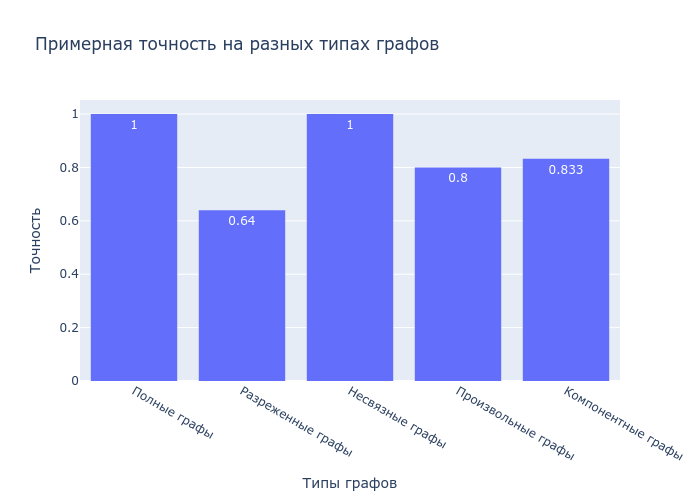
\includegraphics[scale=0.72]{../src/accuracy_plot.png}

Здесь компонентные -- графы, состоящие из двух сильно связных (в смысле количества рёбер) компонент, почти не связанных между собой.

Как мы можем видеть, в тривиальных случаях (полные или несвязные графы) алгоритм даёт точное решение. В то же время, чем меньше становится рёбер в графе (относительно полного графа), тем больше оказывается вероятность ошибки. Это наблюдение можно попробовать объяснить следующим образом: при относительно большем числе рёбер у алгоритма есть больше возможностей исправить свою ошибку выбором нового ребра при выполнении очередной итерации. В то же время, если граф разреженный и мы начали с неудачного остовного дерева, далекого от правильного решения, то может оказаться так, что полностью перестроить граф и получить оптимальное решение мы уже не сможем.

\section{Заключение.}
Рассмотренный алгоритм является оптимальным среди полиномиальных алгоритмов в плане точности, если $\textbf{P} \neq \textbf{NP}$.

На практике оказывается, что такая реализация работает довольно долго даже на графах с не более чем $20$ вершинами (до нескольких минут). Тем не менее, при допустимой ошибке в степени остовного дерева всего лишь на $1$, данное решение сравнимо по времени работы со схожими алгоритмами (например, отличается примерно на $n$ от алгоритма, дающего решение уже с точностью $\log_2n$).

Как мы можем видеть, лучше всего алгоритм работает на графах, в которых доля рёбер (относительно максимально возможного числа) оказывается велика. Тем не менее, даже на разреженных графах алгоритм показывает хорошую точность (по крайней мере в районе $65\%$).


\bibliography{literature}
\bibliographystyle{utf8gost71u}

\end{document}